\documentclass[xcolor=table]{beamer}
\usepackage[UTF8,noindent]{ctexcap}


% 导言区
\title{杂谈勾股定理}
\subtitle{数学史讲座之一}
\institute{方舟科技}
\author{JackLovel}
\date{\today}
\subject{勾股定理}
\keywords{勾股定理,历史}

\logo{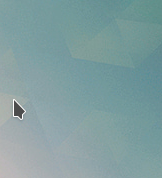
\includegraphics{2.png}}

\newtheorem{thm}{定理}

% 使用主题
\usetheme{AnnArbor} 

% 使用暖色调
\usecolortheme{crane} 
\begin{document}
\begin{frame}
	\titlepage
\end{frame}

\begin{frame}{目录}
  \tableofcontents
\end{frame}

\section{勾股定理在古代}


\begin{frame}
  \frametitle{这是一个标题}
  \framesubtitle{小标题}
  这是简单的一帧
\end{frame}

\begin{frame}
  \frametitle{这是一个标题}
  \framesubtitle{小标题}
  这是简单的一帧
\end{frame}

\begin{frame}{古中国数学}{定理发现}
  中国在3000多年前就知道勾股数的概念,比古希腊更早一些。

  《周髀算经》的记载:
  \begin{itemize}
  \item 公元前 11 世经,商高答周公问:
    \begin{quote}
      勾广三,股修四,径隅五。
    \end{quote}
  \item 又载公元前 7--6 世纪陈子答荣方向。
    \begin{quote}
      若求邪至日者,以日下为勾,日高为股,勾股各自乘,并而开方除之
    \end{quote}
  \end{itemize}
\end{frame}

\begin{frame}
	\begin{thm}
		直角三角形斜边的平方等于两直角边的平方和
	\end{thm}
\end{frame}

\begin{frame}
	\begin{block}{块标题}
		这是一个区块
	\end{block}
\end{frame}

% 图表
\begin{frame}
	有论者认为早在公元前11世纪商高即已证明勾股定理\cite{quanjing}
	\begin{figure}
		\centering
		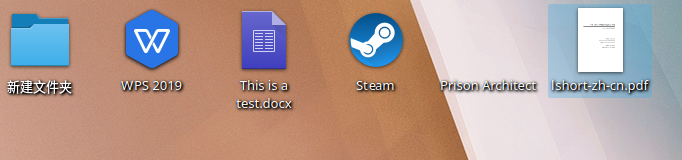
\includegraphics[height=0.4\textheight]{1.png}
		\caption{赵爽的弦图可给出勾股定理的一个}
	\end{figure}
\end{frame}
\end{document}
